\newpage

{ \large \bfseries 3.Αναφορά αποτελεσμάτων – Επιβεβαίωση λειτουργίας }\\ % title 3

\begin{justify}
    Παρακάτω παρουσιάζονται οι κυματομορφές του επεξεργαστή
    που επιβεβαιώνουν την λειτουργία του με όλα τα πιθανά
    \textlatin{Instructions}. Οι εντολές φορτώθηκαν στην μνήμη
    \textlatin{IMEM} μέσω \textlatin{.coe} αρχείων.
\end{justify}

\begin{justify}
    Αρχικά το πρώτο σετ εντολών, το οποίο δώθηκε, βρίσκεται
    στο αρχείο \textlatin{Initialization.coe} και περιέχει τις εξής
    εντολές:\\\\
    \textlatin{1.li r1,6}\\
    \textlatin{2.li r2,6}\\
    \textlatin{3.add r1,r3,r2}\\
    \textlatin{4.bne r1,r2, 0}\\
    \textlatin{5.beq r1,r2, 0}
\end{justify}

\begin{figure}[h]
    \raggedright
    \hspace{-1cm}
    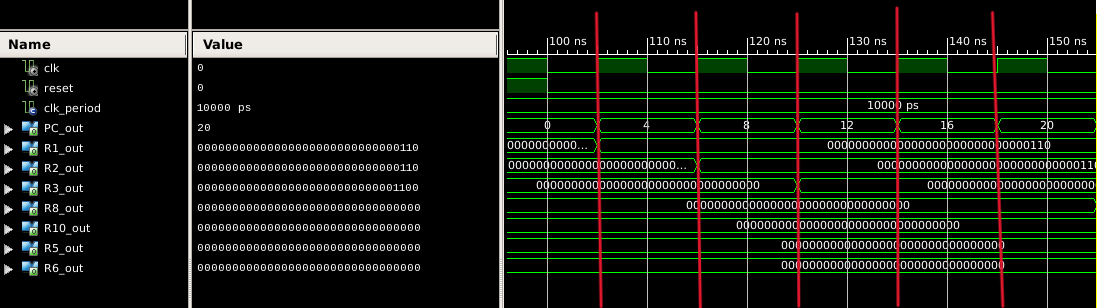
\includegraphics[width=1.1\textwidth]{Images/Screenshot_1.png} % Adjust width as needed
\end{figure}

\begin{justify}
    Για να επιβεβαιώσουμε την λειτουργία του επεξεργαστή
    βλέπουμε τις εξόδους των καταχωρητών στην θετική
    ακμή του ρολογιού. (Όταν δηλαδή περνάνε τα
    αποτελέσματα στην έξοδο).
    Αρχικά το σήμα \textlatin{Reset} είναι ενεργό
    οπότε όλες οι εξόδοι μηδενίζονται. Έπειτα εκτελούνται
    σειριακά οι παραπάνω εντολές (o \textlatin{PC} αυξάνεται
    κατά 4 σε κάθε κύκλο) και έχουμε τα εξής αποτελέσματα
    (με κόκκινο χρώμα φαίνεται ο κάθε κύκλος):\\
    1. Καταχωρείται στον \textlatin{R1} το 6.\\
    2. Καταχωρείται στον \textlatin{R2} το 6.\\
    3. Στον \textlatin{R3} καταχωρείται το αποτέλεσμα
    του αθροίσματος των \textlatin{R1} και \textlatin{R2}.\\
    4. Τα \textlatin{R1} και \textlatin{R2} είναι διαφορετικά
    οπότε η εκτέλεση του προγράμματος συνεχίζεται κανονικά.
    5. Τα \textlatin{R1} και \textlatin{R2} είναι ίσα οπότε
    η εκτέλεση του προγράμματος πρέπει να μεταφερθεί στην θέση
    \textlatin{PC+4+Immediate} (στην περίπτωση μας 0) οπότε
    συνεχίζεται κανονικά.
\end{justify}

\begin{justify}
    Συνεχίζουμε με τις εντολές:\\\\
    \textlatin{1. lui r8,4}\\
    \textlatin{2. lui r10,16}\\
    \textlatin{3. or r8,r5,r10}\\
    \textlatin{4. rol r5,r6,1}\\
    \textlatin{5. ror r6,r5,1}\\
    \textlatin{6. sw r5,4(r10)}
\end{justify}

\newpage

\begin{figure}[h]
    \raggedright
    \hspace{-1cm}
    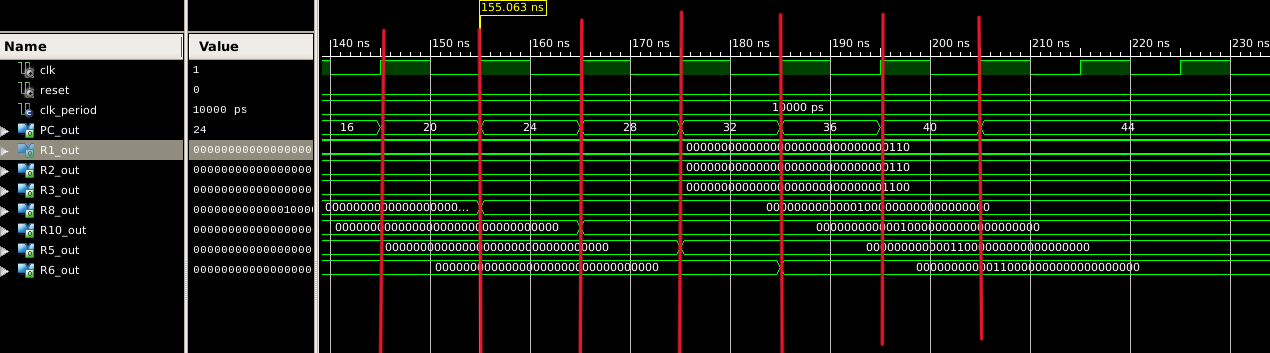
\includegraphics[width=1.1\textwidth]{Images/Screenshot_2.png} % Adjust width as needed
\end{figure}

\begin{justify}
    Στο παραπάνω σετ εντολών βλέπουμε τα εξής:\\
    1. Στον \textlatin{R8} καταχωρείται το 4.\\
    2. Στον \textlatin{R10} καταχωρείται το 16.\\
    3. Στον \textlatin{R5} καταχωρείται το αποτέλεσμα
    του \textlatin{OR} των \textlatin{R8} και \textlatin{R10}.\\
    4. O \textlatin{R5} γίνεται \textlatin{Rotate Left} κατά 1 και
    αποθηκεύεται το αποτέλεσμα στον \textlatin{R6}.\\
    5. Ο \textlatin{R6} γίνεται \textlatin{Rotate Right} κατά 1
    και αποθηκεύεται το αποτέλεσμα στον \textlatin{R5}.\\
    6. Aποθηκεύει την τιμή του \textlatin{10} στην διεύθυνση
    [τιμή\textlatin{R5+4}] όπου αυτο βγαίνει στην πρώτη θέση της μνήμης
    πράγμα που επιβεβαιώνεται αμα ανοίξουμε την μνήμη όπως
    φαίνεται παρακάτω.
\end{justify}

\begin{figure}[h]
    \centering
    \hspace{-1cm}
    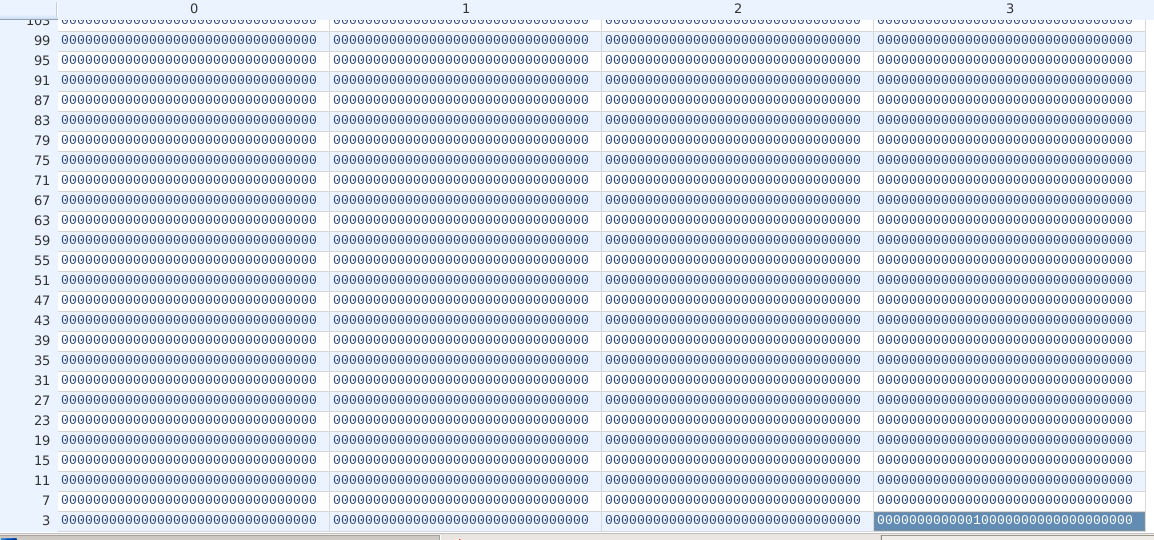
\includegraphics[width=1\textwidth]{Images/Screenshot_3.png} % Adjust width as needed
\end{figure}

\begin{justify}
    Στην συνέχεια επεκτάθηκε το αρχείο \textlatin{Initialization.coe}
    ώστε να επιβεβαιωθεί και η λειτουργία
    των υπόλοιπων εντολών. Οι εντολές που προστέθηκαν είναι:\\\\
    \textlatin{1. and r1,r4,r3}\\
    \textlatin{2. sub r2,r1,r4}\\
    \textlatin{3. sra r1,r1}\\
    \textlatin{4. addi r2,r4,4}\\
    \textlatin{5. beq r4,r3,0}\\
    \textlatin{6. bne r4,r3,0}
\end{justify}

\newpage

\begin{figure}[h]
    \raggedright
    \hspace{-1cm}
    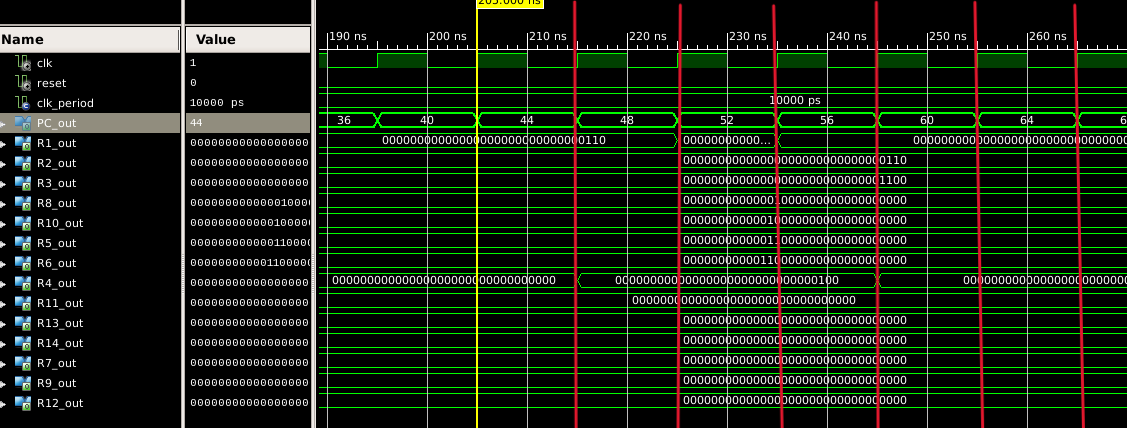
\includegraphics[width=1.1\textwidth]{Images/Screenshot_4.png} % Adjust width as needed
\end{figure}


\begin{justify}
    Στο παραπάνω σετ εντολών βλέπουμε τα εξής:\\
    1. Στον \textlatin{R4} καταχωρείται το αποτέλεσμα
    του \textlatin{AND} των \textlatin{R1} και \textlatin{R3}.\\
    2. Στον \textlatin{R1} καταχωρείται το αποτέλεσμα
    της αφαίρεσης των \textlatin{R2} και \textlatin{R4}.\\
    3. Ο \textlatin{R1} γίνεται \textlatin{Shift Right Arithmetic} κατά 1.\\
    4. Στον \textlatin{R4} καταχωρείται το αποτέλεσμα
    της πρόσθεσης του \textlatin{R2} και του \textlatin{Immediate}.\\
    5. Τα \textlatin{R4} και \textlatin{R3} είναι ίσα
    οπότε η εκτέλεση του προγράμματος συνεχίζεται κανονικά.\\
    6. Τα \textlatin{R4} και \textlatin{R3} είναι διαφορετικά
    οπότε η εκτέλεση του προγράμματος πρέπει να μεταφερθεί στην θέση
    \textlatin{PC+4+Immediate} (στην περίπτωση μας 0) οπότε
    συνεχίζεται κανονικά.
\end{justify}

\begin{justify}
    Συνεχίζουμε με τις εντολές:\\\\	 
    \textlatin{1. not r1,r11}\\ 
    \textlatin{2. sll r11,r13}\\
    \textlatin{3. srl r2, r14}\\
    \textlatin{4. addi r14,r7,4}\\
    \textlatin{5. ori r7,r9,1}
\end{justify}

\begin{figure}[h]
    \raggedright
    \hspace{-1cm}
    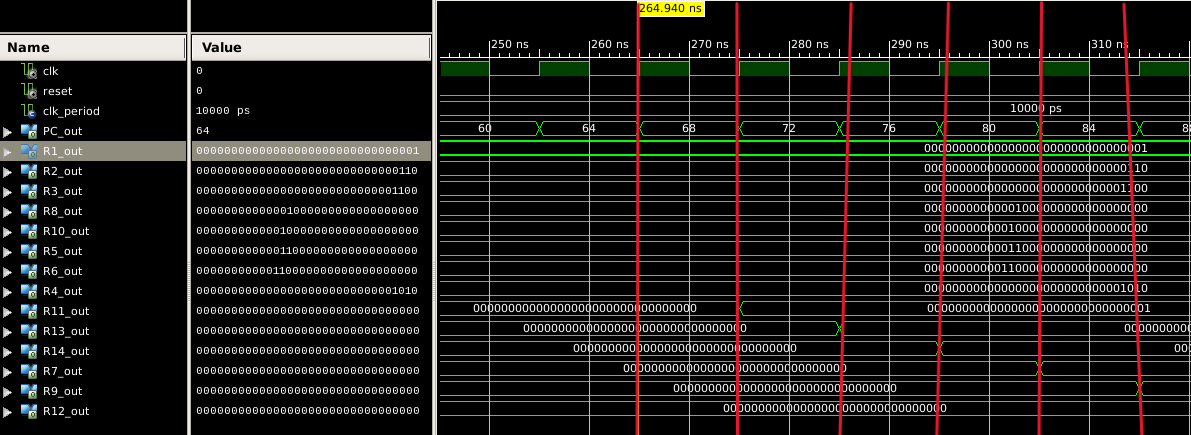
\includegraphics[width=1.1\textwidth]{Images/Screenshot_5.png} % Adjust width as needed
\end{figure}

\newpage

\begin{justify}
    Βλέπουμε τα εξής:\\
    1. Στον \textlatin{R11} καταχωρείται το αποτέλεσμα
    του \textlatin{NOT} του \textlatin{R1}.\\
    2. Ο \textlatin{R11} γίνεται \textlatin{Shift Left Logical} 
    κατά 1 και το αποτέλεσμα αποθηκεύεται στον \textlatin{R13}.\\
    3. Ο \textlatin{R2} γίνεται \textlatin{Shift Right Logical}
    κατά 1 και το αποτέλεσμα αποθηκεύεται στον \textlatin{R14}.\\
    4. Στον \textlatin{R7} καταχωρείται το αποτέλεσμα
    της πρόσθεσης του \textlatin{R14} και του \textlatin{Immediate}.\\
    5. Στον \textlatin{R9} καταχωρείται το αποτέλεσμα
    του \textlatin{OR} των \textlatin{R7} και του \textlatin{Immediate}.
\end{justify}


\begin{justify}
    Και τέλος προσθέσαμε τις εντολές:\\\\  
    \textlatin{1. lw r5,4(r12)}\\
    \textlatin{2. lb r5,4(r11)}\\
    \textlatin{3. b 1}       
\end{justify}

\begin{figure}[h]
    \raggedright
    \hspace{-1cm}
    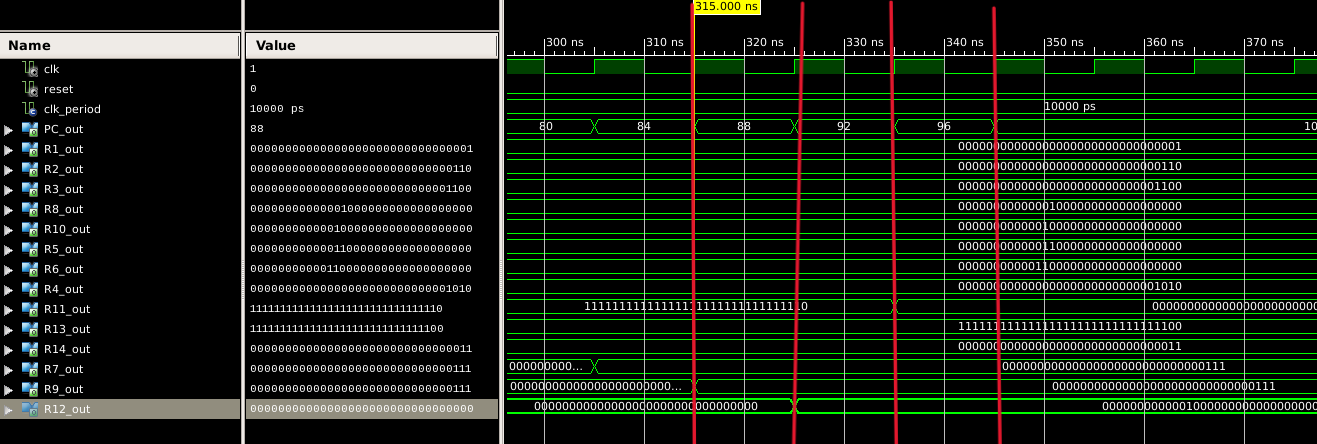
\includegraphics[width=1.1\textwidth]{Images/Screenshot_6.png} % Adjust width as needed
\end{figure}

\begin{justify}
    Και τελικά βλέπουμε τα εξής:\\
    1. Στον \textlatin{R12} καταχωρείται η τιμή της μνήμης
    \textlatin{MEM[0000\_00001]=R10}\\
    2. Στον \textlatin{R11} καταχωρείται η τιμή της μνήμης
    \textlatin{MEM[R5+4]=0}\\
    3. Η εκτέλεση του προγράμματος μεταφέρεται στην θέση
    \textlatin{PC+4+4} που επιβεβαιώνεται αφού
    \textlatin{PC=104}.
\end{justify}